\documentclass[utf8]{book}
\usepackage{titletoc}
\usepackage{titlesec}
\usepackage{ctexcap}
\usepackage[b5paper,text={125mm,195mm},centering,left=1in,right=1in,top=1in,bottom=1in]{geometry}
\usepackage[]{geometry}
\usepackage{imakeidx}
\usepackage{multicol}
\usepackage{hyperref}
\usepackage{graphicx}
\makeindex
\bibliographystyle{plain}
\begin{document}
\title{\heiti Specifying Systems}
\author{First Printing}
\date{2008-2-18}

\frontmatter
\maketitle

\renewcommand\contentsname{目~录}
\tableofcontents

\chapter{\ }
\begin{center}
\huge{\textbf{Specifying Systems}}
\end{center}

\begin{center}
\quad \\ 
\textbf{The TLA+ Language and Tools for} \\
\quad \\ 
\textbf{Hardware and Software Engineers}\\
\quad \\ 
\quad \\ 
\quad \\ 
\quad \\ 
Leslie Lamport\\
\quad \\ 
Microsoft Research\\
\quad \\ 
\quad \\ 
\quad \\ 
\quad \\ 
\quad \\ 

\end{center}


\chapter{序}
过去25年我一直在学习并试图说明和解释并发系统。在这之前,我已经花费很多年学习如何严密的的使用数学方法。我特别感谢在这段时间内帮助我的每一个人,但是我要特别感谢影响我写这本书的两个人。Richard Palais教会了我如何严谨和优雅的使用复杂的数学理论。Martin Abadi影响了TLA的发展,后面的第9节和第10节,也是受到他思想的影响。

目前我知道Mrak Tuttle和Yuan Yu将TLA数学方法用来解决复杂系统工程问题方面做了很多工作。尽管我多次告诉Yuan Yu只是理论不实用,他还是编写了TLC模型检测工具从而将TLA$^+$从理论变成了能解决实际工程问题的理论。在编写了TLA$+$的的语法分析器后,Jean-Charles Gregoire帮助我微调了TLA$+$语言。

感谢下面这些对本书早期版本作出有用评论的人:Dominique Couturier,Douglas Frank,Vinod Grover,David Jefferson,Sara Kalvala 和Wolfgang Schreiner。阅读了所有的草稿并发现了很多错误。Kapila Pahalawatta发现了\textit{ProtoReals}模型中的一个错误。也发现了\textit{ProtoReals}模型中的一个错误,并提出了有效的方法来做呈现。最后特别感谢他认真的阅读了手稿并发现了很多错误。

 \leftline{\qquad \qquad \qquad \qquad \qquad \qquad \qquad \qquad \qquad \qquad \qquad \qquad \textit{Leslie Lamport}} 
 \leftline{\qquad \qquad \qquad \qquad \qquad \qquad \qquad \qquad \qquad \qquad \qquad \qquad  \textit{Palo Alto, California}} 
  \leftline{\qquad \qquad \qquad \qquad \qquad \qquad \qquad \qquad \qquad \qquad \qquad \qquad \textit{4 March 2002}} 
 
\chapter{简介}
这本书将会将会讲解如何使用TLA$+$语言来编写计算系统的说明。虽然这本书很长,但是很对人只需要阅读第一章的83页,这部分包含了工程师所需要掌握的编写系统说明的知识。第一部分适合计算机工程科学的学生,因为只需要相关的工程背景和数学知识便可以学习。第二部分包含了一些针对有经验的读者的复杂理论。本书的剩下部分是一个参考手册,第三部分是关于TLA$+$的工具,第四部分是关于TLA$+$语言本身的。

TLA的官方网页包含了组成本书的一些材料,包含TLA$+$工具,练习、参考著作和一些本书的订正。下面是TLA的网页地址\\
\ \\
\centerline{\textbf{http://lamport.org}}\\

读者可以通过搜索下面的21字符来进行搜索
\begin{figure}[htbp]
\begin{center}
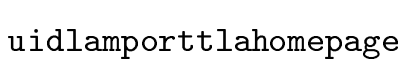
\includegraphics[width=0.4\linewidth]{./fig/fig_0_2.png}
\end{center}
\end{figure}

请不要将这个字符串放在任何的文档否则将会出现在互联网(这里翻译者使用了图片格式,lamport大神首页的邮箱也是图片格式)。\\

\textbf{\large{What Is a Specification?}}\\
\rightline{\textit{\small Writing is nature's way of letting you}}\\
\rightline{\textit{\small know how sloppy your thinking is. }}\\
\rightline{\textit{\small --- Guindon}}\\

说明是描述一个系统如何运转的。说明一个系统可以帮助我们更好的理解系统。设计一个系统之前深刻的理解系统是一个好的主意,那么在实现系统之前写一个系统说明也是一个好的主意。

这本书讲述如何说明一个系统的行为,也就是系统的功能和逻辑。功能和逻辑特性说明一个系统应该做什么。系统还有一些我们不关系的行为,如性能特性。系统的最差性能往往也被用来描述系统的行为特性,例如:第九节解释如何说明一个系统必须在固定长度时间内响应。然而,说明平均性能超过了这里描述的方法的范围。

我们用来编写一个说明是使用数学工具。数学是一种自然的方式可以自己认识到自己的写作是多么草率。使用如英语和汉语不精确的预言很难精确的描述一个问题。在工程中,不精确的表述将会导致严重的错误。为了避免系统中的错误,科学家和工程师豆浆数学作为自己的语言。

本书使用的数学知识比你在课堂学习的数学更加的正式。正式的数学是一种自然的书写让你认识到自己认知的数学是多么的草率。很多数学家和工程师写的数学理论是不精确的,往往只有小部分是精确的,大部分是不精确的。每个等式是一个准确断言,但是你不得不阅读匹配的词语去理解这些等式之间的关系和准确的理解这些等式表述了什么原理。逻辑学家尝试很多方法来消除这些语言,创建正式的数学理论来精确的建模和描述问题。

很多数学家和科学家认为没有单词的正式的数学会冗长和枯燥,它们是错误的。传统数学可以使用一个精确、完备的范式语言来准确的表达。在第11节的\textit{DifferentialEquations}模块,定义梯度等式的解只需要仅仅20几行,如此复杂的数学问题仅仅需要很少的说明。需要最多的是一些很少标准数学概念的简单应用。\\

\textbf{\large{Why TLA$+$?}}\\

我们说明一个系统是通过它被允许的行为进行描述的,即在执行的过程中它会做什么。在1997年,Amir Pnueli提出了使用时态逻辑来描述系统行为。理论上,一个系统都可以使用一个简单的时态逻辑公式来描述。实际中,这是不可能的,Pnueli的时序逻辑引出了描述系统特性的理论,但是不能准确描述系统的所有性能。所以通常通过结合一些传统的方法来进行系统的描述。

20世界80年代后,我发明了基于Pnueli原始逻辑的简单变体TLA---行为的时序逻辑。TLA使得通过简单的公式来描述一个系统成为现实。大多的TLA说明仍然包含了传统和非时序数学,时序逻辑仅仅在描述那些它所擅长描述的行为中起至关重要的作用。TLA提供了优雅的建模方法来解释系统,并且在实际使用中被证明是有效的---也就是众所周知的\textit{断言推理}。然而,这本书是关于如何写系统的说明,不设计到任何的证明。

虽然有很多的方法可以形式化传统的数学,时序逻辑假设了一个基本的逻辑来表述传统的数学。很多计算机科学家往往喜欢用他们喜欢的编程语言。我选择不是很多数学家喜欢的方式---逻辑学家喜欢称它为一阶逻辑和集合论。

TLA提供了描述系统的数学基础。为了编写说明,我们需要建立在这个基础之上的一种完备的语言。我最初思考这种语言应该是一类抽象的编程语言,这种编程语言的语法应该是基于TLA的。我不知道什么样的编程结构是最好的,所以我决定开始直接使用TLA编写说明。令我惊讶的是,我 发现我根本不需要程序化的结构。我需要的仅仅是一种描述数学的健壮语言。

数学家尽管发展了写数学公式的科学,但是它们没有将这种数学科学发展称工程学科。它们仅仅发展出了描述数学的低级抽象符号,但是没有定义数学的高级抽象符号。一个实际系统的说明往往需要好几百页。数学家知道如何写20行的共识而不是20页的公式,所以我不得不提出书写长公式的符号。我从编程语言汲取了想法来编写高度抽象的说明。

我最终将这种语言称为TLA$+$。我在课程中更新了写不同系统的说明书,但是过去几年这个语言基本没有证明变化。我发现TLA$+$对于很多类型的系统都是编写说明很好的方法,从编程接口(APIs)到分布式系统。他可以编写任何一个离散系统的精确、形式化的描述。特别地,非常适合用来描述异步系统---也就是说,系统的组件并不是严格的按照规定的步骤顺序进行执行的。\\

\large{\textbf{关于这本书}}\\

第一部分包含了第1-7节是这本书的核心,建议从前往后认真阅读。解释了如何说明一类性质---安全性质。这些特性是工程师需要了解的,这些特性几乎不需要时序逻辑。

阅读完第一部分后,第二部分每一章节都是彼此独立的,读者可以阅读第二部分自己喜欢的部分。第8节使用了时序逻辑来说明活跃性。第9节描述了如何说明实时性,第10节描述如果组织说说明。第11节包含了更多高级的例子。

第三部分是三个TLA$+$工具的参考手册:语法分析器、TLATEX排版程序和TLC模型检测器。如果你想使用TLA$+$,你将会使用到这三个工具,可以在TLA网站获取。TLC是三者中最复杂的一个,网站上的例子可以教你如何使用,但是你需要阅读第14节学习如何更高效的使用TLC。

第四部分是TLA$+$语言的参考手册。第一部分已经能满足学习编写说明的全部知识。如果你对语法和句法存在疑问可以阅读第四部分。第15节给出了TLA$+$的语法。第16节描述了TLA$+$内建操作符的精确含义和通用形式。第17节描述了所有高层级的TLA$+$结构的准确含义,例如定义。第18节描述了第9节的标准模块(除了实时模块)和第14节的TLC模块。如果你好像如何使用TLA$+$来建模标准的数学元素,你需要阅读本节。

第四部分有一些你不经常使用的东西:一个最小手册压缩很多有用的信息。268-273页列出了TLA$+$的操作,所有用户可定义的符号,所有操作符的优先级,所有标准模块定义的操作符,和符号的ASCII表示。
\mainmatter

\part{让我们开始}
一个系统说明包含需要许多传统数学和很少的一些时序逻辑。也就解释了为什么很多的系统说明还是使用传统数学来描述的。为了编写说明,你还是要熟悉传统的数学。不幸的是,在很多学校的计算机系认为C++的流畅比基础数学的教育更重要。所以,很多读者对用来写说明的数学并不熟悉。好在这些数学知识都很简单。如果C++还没有摧毁你的逻辑思考能力,那么你应该能弥补上你的数学教育。在学习C++之前你可能已经学习了算术,所以我将假设你知道数字和基础的算术知识。我会尝试解释所有你需要的数学概念,从第1节我们从基本的数学元素开始。我希望所有的读者发现这个回顾完全是没有必要的。

在第一章节回顾简单的数学知识后,第2-5节通过一系列的例子来描述TLA$+$。第6节解析一些编写说明的数学知识,第7节回顾之前讲述的并提供一些建议。在完成第7节之后,你可以应对对很多传统工程实际问题的说明。

\chapter{简单数学基础}

\section{命题逻辑}
代数基础是由实数和操作符$+$、$-$、$*$和$/$构成。逻辑命题是由两个逻辑值\textit{TRUE}、\textit{FALSE}和5个操作符构成的。5个操作符是


\subsection{二级节标题}

\subsubsection{三级节标题}

\begin{multicols}{2}

清朝中期, 外国人就开始中国采集植物标本。清朝中期, 外国人就开始中国采集植物标本。清朝中期, 外国人就开始中国采集植物标本。清朝中期, 外国人就开始中国采集植物标本。清朝中期, 外国人就开始中国采集植物标本。清朝中期, 外国人就开始中国采集植物标本。

\end{multicols}

\chapter{植物区系分区}

\section{一级节标题}

\subsection{二级节标题}

\subsubsection{三级节标题}

\begin{multicols}{2}
和标本采集植物调查和标本采集植物调查和标本采集植物调查和标本采集植物调查和标本采集植物调查和标本采集植物调查和标本采集植物调查和标本采集植物调查和标本采集植物调查和标本采集植物调查和标本采集植物调查和标本采集植物调查和标本采集植物调查和标本采集植物调查和标本采集植物调查和标本采集植物调查和标本采集植物调查和标本采集植物调查和标本采集植物调查和标本采集植物\index{调查}和标本采集植物调查和标本采集植物调查和标本采集植物调查和标本采集

\end{multicols}

\part{植物多样性分区概述}

\chapter{东北地区}

\begin{multicols}{2}
Lorem ipsum dolor sit amet, consectetur adipisicing elit, sed do eiusmod tempor incididunt ut labore et dolore magna aliqua. Ut enim ad minim veniam, quis nostrud exercitation ullamco laboris nisi ut aliquip ex ea commodo consequat. Duis aute irure dolor in \index{reprehenderit} in voluptate velit esse cillum dolore eu fugiat nulla pariatur. Excepteur sint occaecat cupidatat non proident, sunt in culpa qui officia deserunt mollit anim id est laborum.
\end{multicols}

\chapter{华北地区}
\begin{multicols}{2}
Lorem ipsum dolor sit amet, consectetur adipisicing elit, sed do eiusmod tempor incididunt ut labore et dolore magna aliqua. Ut enim ad minim veniam, quis nostrud exercitation ullamco laboris nisi ut aliquip ex ea commodo consequat. Duis aute irure dolor in reprehenderit in voluptate velit esse cillum dolore eu fugiat nulla pariatur. Excepteur sint occaecat cupidatat non proident, sunt in culpa qui officia deserunt mollit anim id est laborum.
\end{multicols}

\include{angiosperms}

\appendix

\chapter{APG分类系统的科名}

内容附录内容附录内容附录内容附录内容附录内容附录内容附录内容附录内容附录内容附录内容附录内容附录内容附录内容附录内容附录内容附录内容附录内容文内容正文内容正文内容正文\index{内容}

内容附录内容附录内容附录内容附录内容附录内容附录内容附录内容附录内容附录内容附录内容附录内容附录内容附录内容附录内容附录内容附录内容附录内容附录内容附录内容附录内容正文内容正文\cite{DK1}.

\renewcommand\indexname{索~~引}
\printindex
\addcontentsline{toc}{chapter}{索~引}

\backmatter

\addcontentsline{toc}{chapter}{参考文献}

\begin{thebibliography}{参考文献}
\bibitem[Knuth1 et al. 1997]{DK1} D. Knuth, T.A.O.C.P. , Vol. 1, Addison-Wesley, 1997.
\bibitem[Knuth2]{DK2} D. Knuth, T.A.O.C.P. , Vol. 2, Addison-Wesley, 1997.
\bibitem[TONG YH 2014]{TONG} TONG YH, PANG KS, XIAN NH, 2014. Carpinus insularis (Betulaceae), A new species from Hong Kong [J]. J Trop Subtrop Bot, 22(2): 121-124. [童毅华, 彭权森, 夏念和,2014. 香港桦木科一新种——香港鹅耳枥 [J]. 热带亚热带植物学报,22(2):121-124.]
\bibitem[XIA NH 2008]{XIA} XIA NH, DENG YF, YIP KL, 2008. Syzygium impressum (Myrtaceae), A new species from Hong Kong [J]. J Trop Subtrop Bot, 16(1):19-22. [夏念和,邓云飞,叶国梁,2008. 香港桃金娘科一新种-凹脉赤楠 [J].热带亚热带植物学报,16(1):19-22.]
\end{thebibliography}

\chapter{后~~记}

后记内容后记内容后记内容后记内容后记内容后记内容后记内容后记内容后记内容后记内容后记内容后记内容后记内容后记内容后记内容后记内容后记内容后记内容后记内容后记内容后记内容后记内容后记内容后记内容后记内容后记内容后记内容后记内容后记内容后记内容后记内容后记内容后记内容后记内容后记内容后记内容后记内容后记内容后记内容后记内容后记内容后记内容后记内容后记内容后记内容后记内容后记内容后记内容后记内容后记内容后记内容后记内容后记内容后记内容后记内容后记内容后记内容后记内容后记内容后记内容后记内容后记内容后记内容后记内容后记内容

\begin{flushright}
作~~者~~~~~~~~~

2018年1月~~~~~
\end{flushright}

\end{document}
